\documentclass[tikz,border=10pt]{standalone}

% Packages
\usepackage{tikz}
\usetikzlibrary{shapes.geometric, arrows.meta, positioning}

% TikZ Styles
\tikzset{
    block/.style={
        rectangle,
        minimum width=2.8cm,
        minimum height=1.2cm,
        text centered,
        draw=black,
        rounded corners
    },
    attentionblock/.style={
        rectangle,
        minimum width=3.8cm,
        minimum height=1.6cm,
        text centered,
        draw=orange!80,
        fill=orange!20,
        very thick,
        rounded corners
    },
    modelblock/.style={
        rectangle,
        minimum width=4.8cm,
        minimum height=2cm,
        text centered,
        draw=blue!70,
        fill=blue!10,
        very thick,
        rounded corners
    },
    arrow/.style={
        thick,
        ->,
        >=Stealth
    }
}

\begin{document}

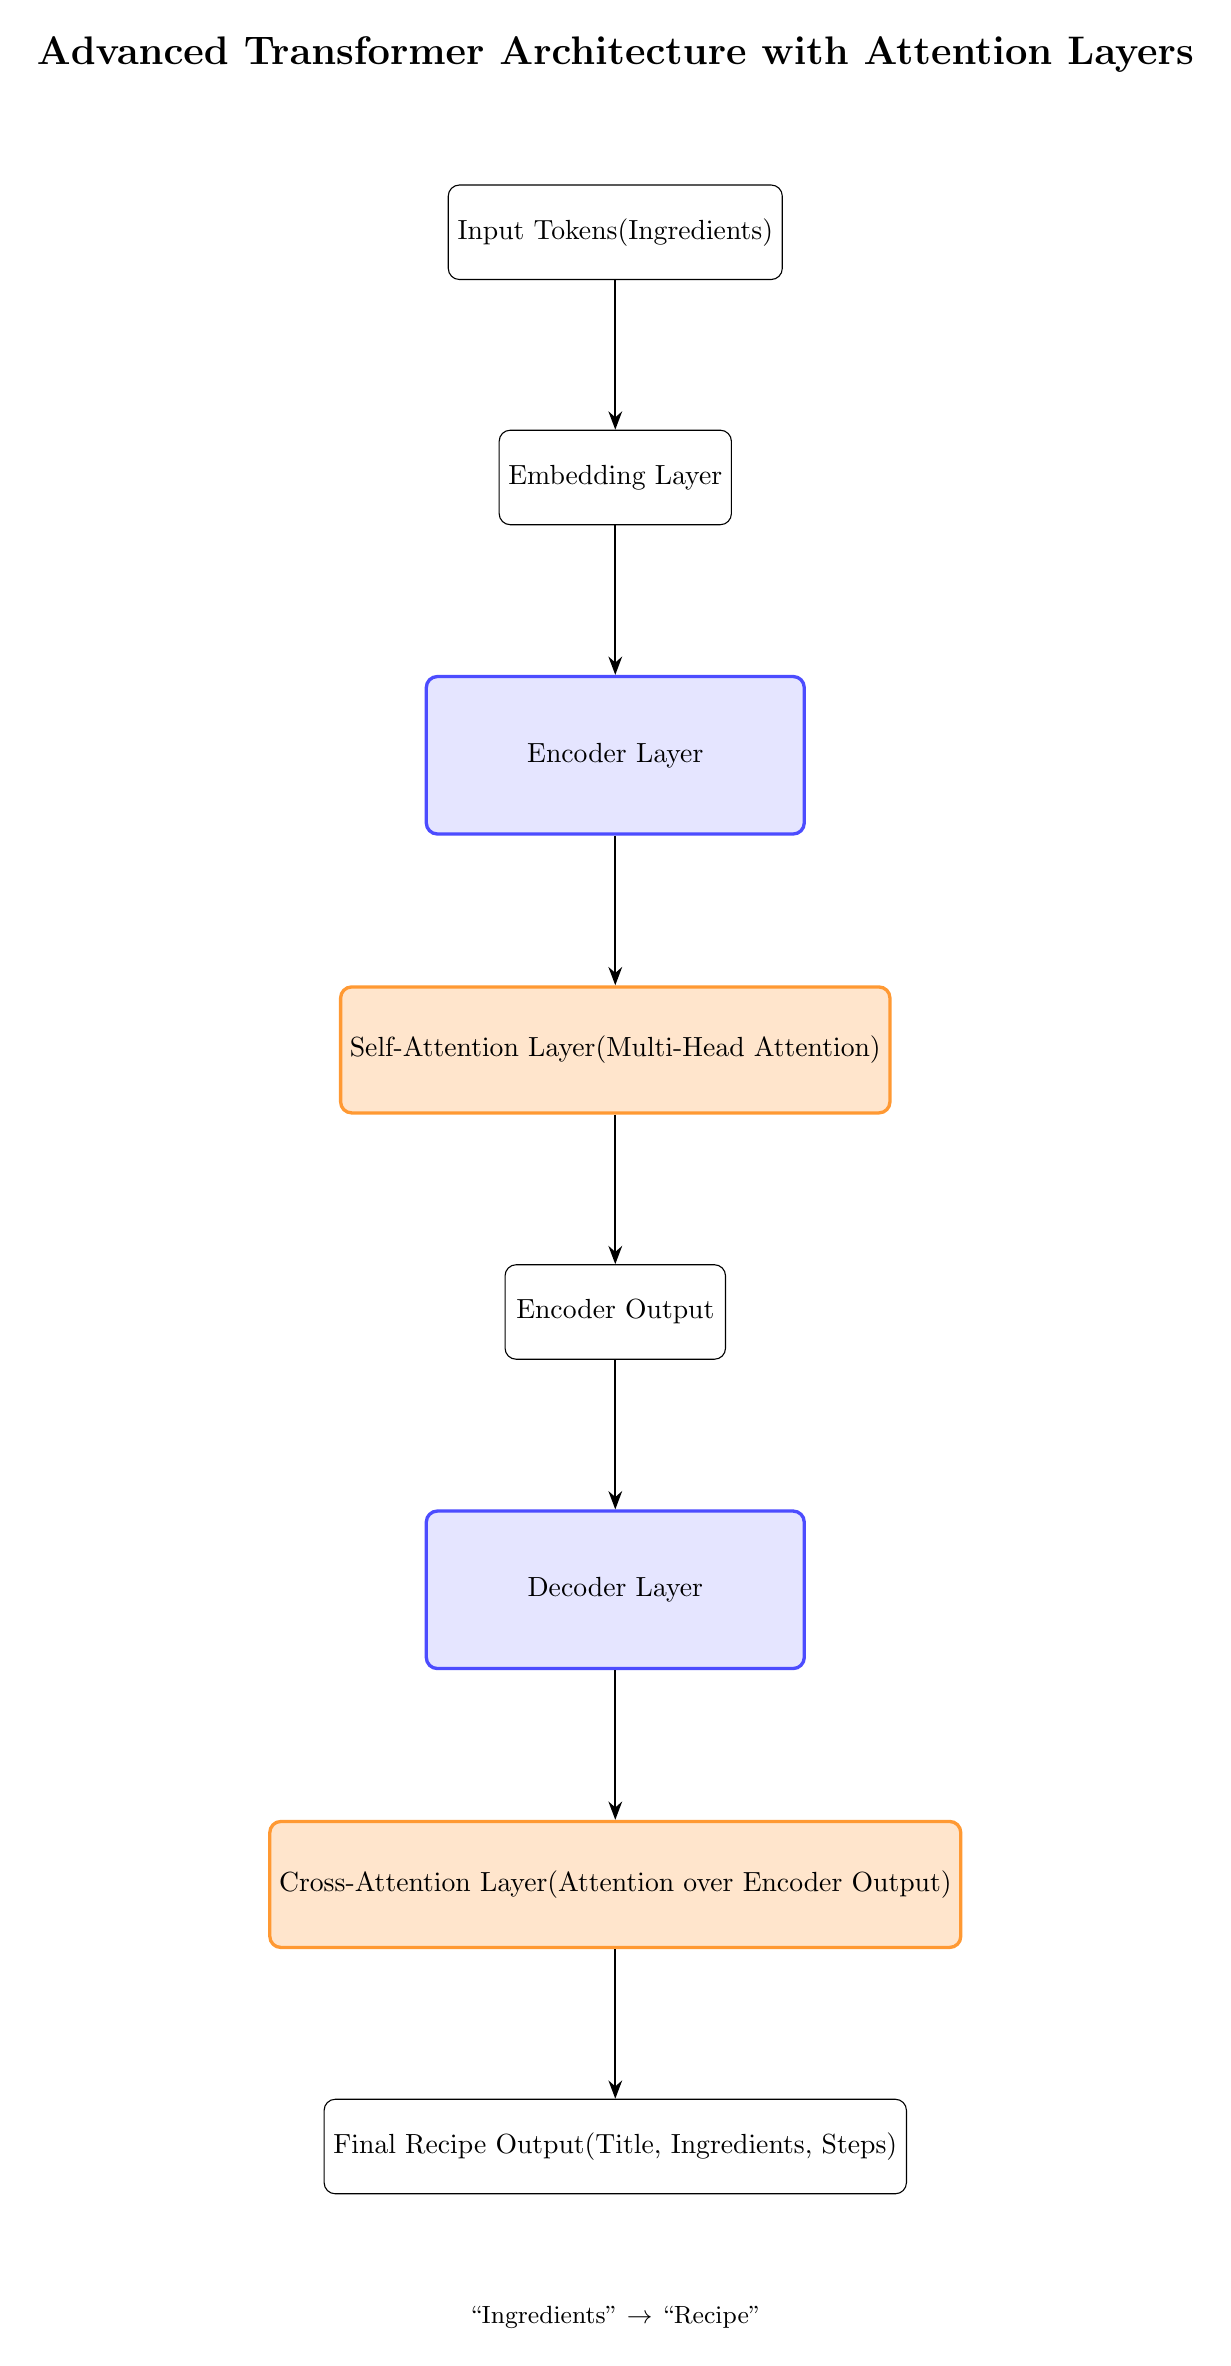
\begin{tikzpicture}[node distance=1.9cm]

% Nodes
\node (input) [block] {Input Tokens \\ (Ingredients)};
\node (embedding) [block, below=of input] {Embedding Layer};
\node (encoder) [modelblock, below=of embedding] {Encoder Layer};
\node (selfattention) [attentionblock, below=of encoder] {Self-Attention Layer \\ (Multi-Head Attention)};
\node (encoderoutput) [block, below=of selfattention] {Encoder Output};
\node (decoder) [modelblock, below=of encoderoutput] {Decoder Layer};
\node (decoderattention) [attentionblock, below=of decoder] {Cross-Attention Layer \\ (Attention over Encoder Output)};
\node (finaloutput) [block, below=of decoderattention] {Final Recipe Output \\ (Title, Ingredients, Steps)};

% Arrows
\draw[arrow] (input) -- (embedding);
\draw[arrow] (embedding) -- (encoder);
\draw[arrow] (encoder) -- (selfattention);
\draw[arrow] (selfattention) -- (encoderoutput);
\draw[arrow] (encoderoutput) -- (decoder);
\draw[arrow] (decoder) -- (decoderattention);
\draw[arrow] (decoderattention) -- (finaloutput);

% Title
\node[above=1.3cm of input] {\Large \textbf{Advanced Transformer Architecture with Attention Layers}};

% Caption
\node[below=1.3cm of finaloutput] {\small ``Ingredients'' $\rightarrow$ ``Recipe''};

\end{tikzpicture}

\end{document}